\chapter{Controlling Vehicle Tools}

So far a control system for vehicles is implemented with a GUI. This chapter takes a look on how to proceed with embedding the control system of the associated tools from a vehicle. Since only one model contains an end-effector, the generalised system will be based on the serial manipulator model.

\section{Serial Manipulator}

The \Cref{fig:KinematicsSerialManipulator} represents how the forward and inverse kinematics works in the implemented model. Also, an illustration of the communication between each joint is conducted. This is done by having variables of the position, rotation and angle on each part of the model. The angle is set by linking the respective parts from the base. A control interface for a tool with inverse and forward kinematics can be applied to any models given with a base and an end-effector. 


\begin{figure}[ht]
    \centering
    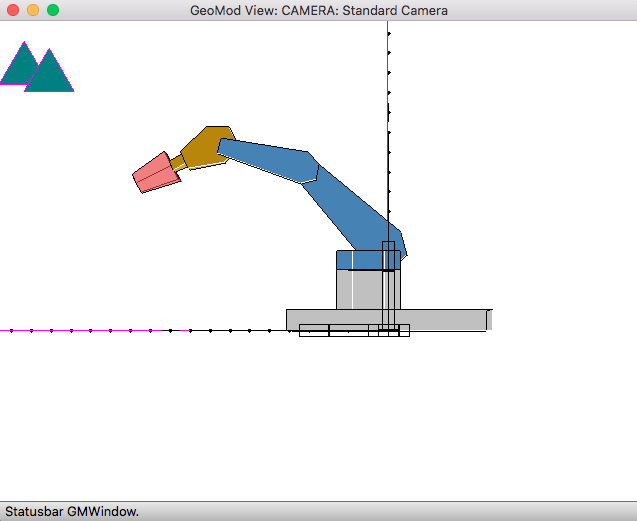
\includegraphics[height=8cm]{images/GeometricModel.png}
    \caption[Geometric model of a serial manipulator]{Geometric model of a serial manipulator}
    \label{fig:SerialManipulator}
\end{figure}


\section{Kinematics}
It was mentioned that from the work of Martin Lygre Fuglevik, the control system for desired position and orientation of objects along a network of paths was partially implemented. Most of the implementation worked as it should, but some occurrence regarding rotation in motion to a particular path did not work as prompted. Some small alteration had to be done in the model in order to continue the implementation of the control system. 

\begin{figure}[ht]
    \centering
    \includegraphics[height=7cm]{images/Diagram_Serial_Manipulator.png}
    \caption[Kinematic connection of  each part of the serial manipulator model]{Kinematic connection of  each part of the serial manipulator model}
    \label{fig:KinematicsSerialManipulator}
\end{figure}


The \Cref{fig:KinematicsSerialManipulator} illutrates how the forward and inverse kinematics works on the implemented model. This is done by having variables over the position, rotation and angle on each part of the model. The angle is determined by linking the parts from the base. By applying forward kinematics, the joints angle is independently controlled for each parts beginning from the position of the linked mechanism, the bracket, to end-effector, the gripper. The function \textit{dirKin()} is an already implemented function that calculate joint angels of all the joints, when one of the joints is moved. This makes a lot of unnecessary computation regarding to joints that are not affected of certain movement. This was disregarded as it did not prevent the objective of this project, but should be taken into account in future for optimization. Forward kinematics works well for a desired end position for the end-effector, but is rather impractical to control when following a path.

With inverse kinematics, the position of the base and joint angle is determined from the position of the gripper. Working with inverse kinematics makes it possible to have a desired position for the gripper while the base is under displacement as long it is within the workspace. Note, it also applies to a displacement of a path. This method of control is very helpful for a UAV, considering currents and other disturbances in the sea. Also, moving a tool along a path can be achieved, as the joints angle is calculated and set during the series of translation and rotation of the gripper. 

\begin{figure}[ht]
  \centering
  \subfloat[Forward kinematics]{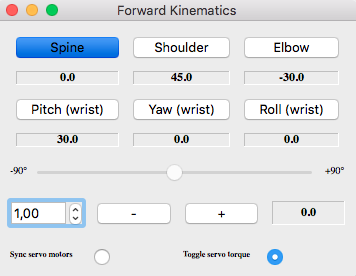
\includegraphics[width=0.31\textwidth]{images/forward.png}\label{fig:forward}}
  \hfill
  \subfloat[Inverse kinematics]{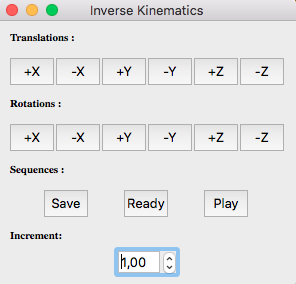
\includegraphics[width=0.31\textwidth]{images/inverse.png}\label{fig:inverse}}
  \hfill
  \subfloat[Motion control]{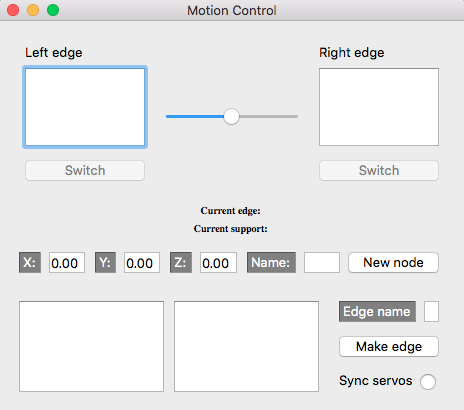
\includegraphics[width=0.31\textwidth]{images/Motion.png}\label{fig:motion}}
  \caption[Control panels implemented by Martin Lygre Furevik]{Control panels implemented by Martin Lygre Furevik}
  \label{fig:martincontrolpanels}
\end{figure}

The implementation of the inverse kinematics solver for this specific model was developed by Sven Fjeldaas \cite{sven}. In Martin Lygre Fureviks master thesis, the inverse kinematics solver was implemented in the model with a corresponding control panel for the inverse kinematics. A similar control panel for forward kinematics was also made for the model. In addition, a motion controller for the robot was created to move the gripper along a path. The controls for the forward, inverse kinematics and motion can be seen in \Cref{fig:martincontrolpanels}.  The great thing about the implementation of the motion controller is it requires a tool and a path. This is done by connecting a pointer to the tool variable from an end-effector model, like the gripper, and a pointer to the path variables from a model. Any given model can, therefore, be freely moved along a given path. For tools, the motion on the path calls the inverse kinematics implemented in the model to regulate the relation between the vehicle and the tool. Combining the motion controller with the implemented control system during this project, tracking a path while the base is in motion is now possible to demonstrate in GeoMod (\Cref{fig:displacement}). 


\begin{figure}[ht]
  \centering
  \subfloat[The gripper is following a path]{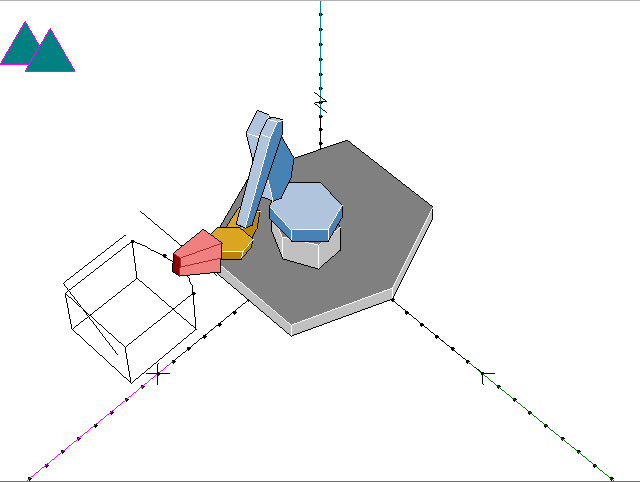
\includegraphics[width=0.4\textwidth]{images/serial_1.png}\label{fig:s1}}
  \hfill
  \subfloat[The gripper is still following the path, during displacement]{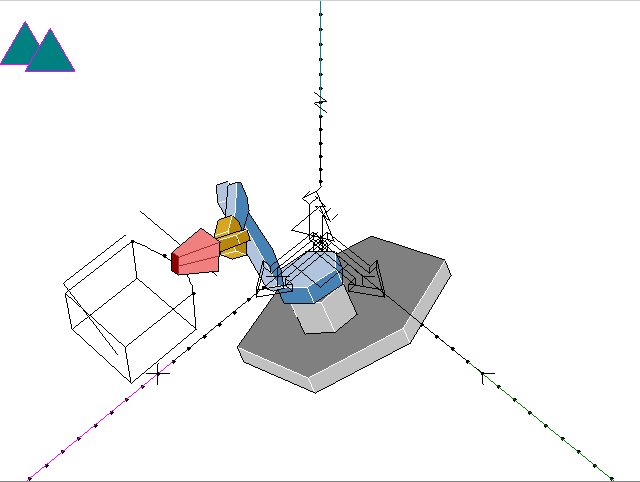
\includegraphics[width=0.4\textwidth]{images/serial_2.png}\label{fig:s2}}
  \caption[Displacement of the base of serial manipulator model]{Displacement of the base of the serial manipulator model}
  \label{fig:displacement}
\end{figure}